\documentclass[border=3pt]{standalone}
\usepackage[T1]{fontenc}
\usepackage{lmodern}
\usepackage{amsmath,amssymb}
\usepackage{xcolor}
\usepackage{tikz}
\usetikzlibrary{positioning,arrows.meta,fit,backgrounds,calc,shapes.misc}
% Notation for emission factors, marginal emissions, carbon prices and border charges.
\newcommand{\edec}{e_{\mathrm{dec}}}
\newcommand{\eall}{e_{\mathrm{all}}}
\newcommand{\eout}{e_{\mathrm{out}}}
\newcommand{\ein}{e_{\mathrm{in}}}
\newcommand{\Ex}{E_{x}}
\newcommand{\Em}{E_{m}}
\newcommand{\pX}{p_{x}}
\newcommand{\pM}{p_{m}}
\newcommand{\tauref}{\tau^{\mathrm{ref}}}
\newcommand{\cgross}{c_{\mathrm{gross}}}
\newcommand{\rhostar}{\rho^{\star}}
\newcommand{\tco}{tCO$_2$}

\DeclareMathSizes{10}{10}{7.5}{7.5}
\DeclareMathSizes{9.5}{9.5}{7.5}{7.5}
\DeclareMathSizes{8.5}{8.5}{7.1}{7.1}
% Grey-scale redundancy: exporter node double border, other-price node dashed border, EU nodes solid.
% Figure 1 of the paper: intervention -> rerouting -> zonal output -> local emissions -> carbon-group accounting.
% Build: pdflatex fig_schematic.tex (in paper/figs).
% Natural width about 150 mm (the text width), so the smallest text stays at or above 7 pt.
\definecolor{eufill}{HTML}{E3EFF6}\definecolor{euline}{HTML}{245A73}
\definecolor{xfill}{HTML}{F6E3CF}\definecolor{xline}{HTML}{9A5B1E}
\definecolor{ofill}{HTML}{ECECEC}\definecolor{oline}{HTML}{6B6B6B}
\definecolor{rulefill}{HTML}{F2D29B}\definecolor{ruleline}{HTML}{8C5A16}
\definecolor{ink}{HTML}{202020}\definecolor{flow}{HTML}{2E7D32}
\newcommand{\ttl}[1]{{\fontsize{10}{12}\selectfont\bfseries #1}}
\newcommand{\ttlf}{\fontsize{10}{12}\selectfont\bfseries}
\newcommand{\eqs}{\fontsize{9.5}{11.5}\selectfont}
\newcommand{\sml}{\fontsize{8.5}{10}\selectfont}
\begin{document}
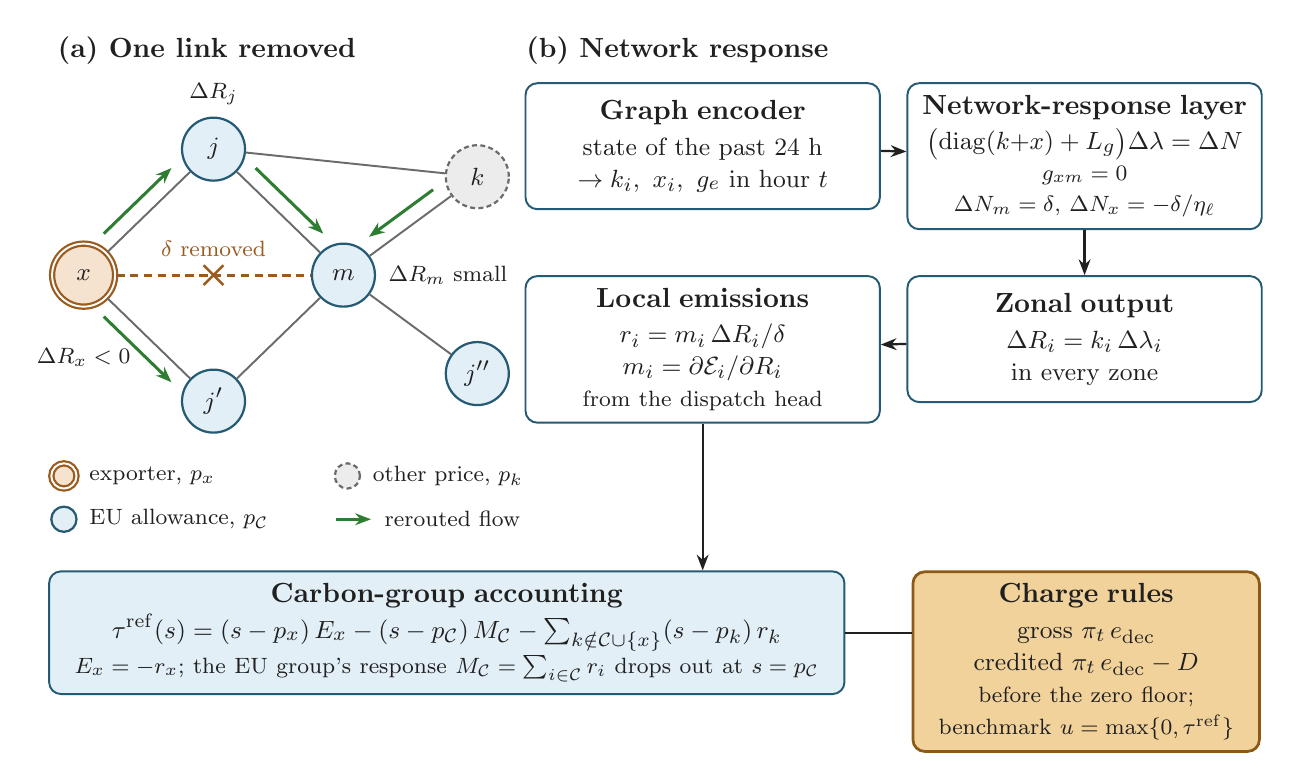
\begin{tikzpicture}[
  text=ink, font=\eqs,
  zn/.style={circle, minimum size=8mm, inner sep=0pt, line width=0.8pt, font=\eqs},
  eu/.style={zn, draw=euline, fill=eufill},
  ex/.style={zn, draw=xline, fill=xfill, double=white, double distance=0.7pt},
  ot/.style={zn, draw=oline, fill=ofill, dash pattern=on 1.8pt off 1.2pt},
  ln/.style={line width=0.7pt, draw=oline},
  rr/.style={-{Stealth[length=2mm]}, line width=1.1pt, draw=flow},
  stp/.style={rounded corners=1.5mm, draw=euline, fill=white, line width=0.7pt, align=center,
              inner sep=1.5mm, text width=42mm, minimum height=16mm},
  arr/.style={-{Stealth[length=2mm]}, line width=0.8pt, draw=ink},
]
% ---------------- (a) one link removed, energy rerouted ----------------
\node[anchor=west, font=\ttlf] at (-0.45,2.85) {(a) One link removed};
\node[ex] (x) at (0,0) {$x$};
\node[eu] (m) at (3.3,0) {$m$};
\node[eu] (j1) at (1.65,1.6) {$j$};
\node[eu] (j2) at (1.65,-1.6) {$j'$};
\node[ot] (k) at (5.0,1.25) {$k$};
\node[eu] (j3) at (5.0,-1.25) {$j''$};
\draw[ln] (x) -- (j1); \draw[ln] (x) -- (j2); \draw[ln] (j1) -- (m); \draw[ln] (j2) -- (m);
\draw[ln] (m) -- (k); \draw[ln] (m) -- (j3); \draw[ln] (j1) -- (k);
\draw[line width=1.0pt, draw=xline, dash pattern=on 3pt off 2pt] (x) -- (m)
  node[midway, draw=xline, line width=0.9pt, cross out, minimum size=2.2mm, inner sep=0pt, solid] {};
\node[font=\sml, text=xline] at (1.65,0.34) {\mbox{$\delta$ removed}};
% rerouted flows: each arrow runs parallel to its link, offset by 2 mm, from 5.5 mm off one node centre to 5.5 mm off
% the other (calc: point along the link, then 2 mm along the link direction turned by +-90 degrees)
\draw[rr] ($(x)!5.5mm!(j1)!2mm!90:(j1)$) -- ($(j1)!5.5mm!(x)!2mm!-90:(x)$);
\draw[rr] ($(j1)!5.5mm!(m)!2mm!90:(m)$) -- ($(m)!5.5mm!(j1)!2mm!-90:(j1)$);
\draw[rr] ($(k)!5.5mm!(m)!2mm!-90:(m)$) -- ($(m)!5.5mm!(k)!2mm!90:(k)$);
\draw[rr] ($(x)!5.5mm!(j2)!2mm!-90:(j2)$) -- ($(j2)!5.5mm!(x)!2mm!90:(x)$);
\node[font=\sml] at (0,-1.05) {\mbox{$\Delta R_x<0$}};
\node[font=\sml, anchor=west] at (3.75,0) {\mbox{$\Delta R_m$ small}};
\node[font=\sml] at (1.65,2.3) {\mbox{$\Delta R_j$}};
% legend
\node[ex, minimum size=3.2mm] at (-0.25,-2.55) {};
\node[anchor=west, font=\sml] at (-0.05,-2.55) {exporter, $\pX$};
\node[eu, minimum size=3.2mm] at (-0.25,-3.1) {};
\node[anchor=west, font=\sml] at (-0.05,-3.1) {EU allowance, $p_{\mathcal{C}}$};
\node[ot, minimum size=3.2mm] at (3.35,-2.55) {};
\node[anchor=west, font=\sml] at (3.55,-2.55) {other price, $p_k$};
\draw[rr] (3.2,-3.1) -- (3.65,-3.1);
\node[anchor=west, font=\sml] at (3.7,-3.1) {rerouted flow};

% ---------------- (b) model chain ----------------
\begin{scope}[xshift=5.6cm]
\node[anchor=west, font=\ttlf] at (-0.1,2.85) {(b) Network response};
\node[stp, anchor=north west] (s1) at (0,2.45)
  {\ttl{Graph encoder}\\[0.5mm] state of the past 24~h\\ \mbox{$\to k_i,\ x_i,\ g_e$ in hour $t$}};
\node[stp, anchor=north west] (s2) at (4.85,2.45)
  {\ttl{Network-response layer}\\[0.5mm] \mbox{$\bigl(\operatorname{diag}(k{+}x)+L_g\bigr)\Delta\lambda=\Delta N$}\\[0.3mm]
   {\sml \mbox{$g_{xm}=0$}\\ \mbox{$\Delta N_m=\delta$, $\Delta N_x=-\delta/\eta_\ell$}}};
\node[stp, anchor=north west] (s3) at (4.85,0.0)
  {\ttl{Zonal output}\\[0.5mm] \mbox{$\Delta R_i=k_i\,\Delta\lambda_i$}\\ in every zone};
\node[stp, anchor=north west] (s4) at (0,0.0)
  {\ttl{Local emissions}\\[0.5mm] \mbox{$r_i=m_i\,\Delta R_i/\delta$}\\ \mbox{$m_i=\partial\mathcal{E}_i/\partial R_i$}\\ {\sml from the dispatch head}};
\draw[arr] (s1) -- (s2);
\draw[arr] (s2) -- (s3);
\draw[arr] (s3) -- (s4);
\end{scope}

% ---------------- bottom row: accounting and comparison ----------------
\node[rounded corners=1.5mm, draw=euline, fill=eufill, line width=0.7pt, align=center, inner sep=1.5mm,
      text width=98mm, anchor=north west] (s5) at (-0.45,-3.75)
  {\ttl{Carbon-group accounting}\\[0.5mm]
   \mbox{$\tauref(s)=(s-\pX)\,\Ex-(s-p_{\mathcal{C}})\,M_{\mathcal{C}}-\sum_{k\notin\mathcal{C}\cup\{x\}}(s-p_k)\,r_k$}\\[0.4mm]
   {\sml \mbox{$\Ex=-r_x$; the EU group's response $M_{\mathcal{C}}=\sum_{i\in\mathcal{C}}r_i$ drops out at $s=p_{\mathcal{C}}$}}};
\node[rounded corners=1.5mm, draw=ruleline, fill=rulefill, line width=1.0pt, align=center, inner sep=1.5mm,
      text width=41mm, anchor=north east] (s6) at (14.95,-3.75)
  {\ttl{Charge rules}\\[0.5mm] \mbox{gross $\pi_t\,\edec$}\\ \mbox{credited $\pi_t\,\edec-D$}\\ {\sml \mbox{before the zero floor;}}\\ {\sml \mbox{benchmark $u=\max\{0,\tauref\}$}}};
\draw[arr] (s4.south) -- (s4.south |- s5.north);
\draw[line width=0.6pt, draw=ink] (s5.east) -- (s5.east -| s6.west);
\end{tikzpicture}
\end{document}
